\section{Graphical User Interface (GUI)}

Due to being an extension of the existing MNE-CPP project, no new GUI is needed. Nevertheless the new features must be integrated into Disp3D and MNE Scan. \\

Disp3D acts as a test environment with a basic interface. It loads sample data and features various graphical options. \\
The new functions are executable through the GUI of Disp3D. For that, a new item is created to expand the existing product. (\ref{integration}) \\ 
	
\begin{wrapfigure}{L}{0.25\textwidth}
	
	\begin{center}
		
		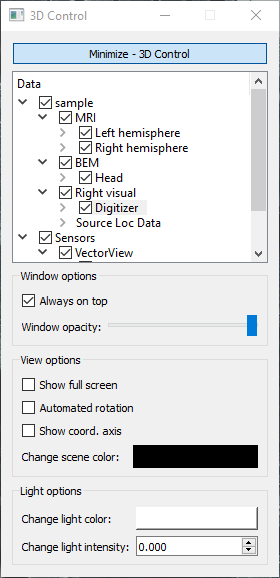
\includegraphics[scale=0.5]{Figures/Disp3D.PNG}
	
	\end{center}
	
	\caption{Disp3D}

\end{wrapfigure}
~\\
~\\
Further the MNE-CPP project consists of 3 big standalone programs, namely MNE Scan, MNE Analyze and MNE Browse, which can be accessed by a main launcher. Alongside Disp3D, the new features are executable through the MNE Scan application.

\begin{wrapfigure}{R}{1.30\textwidth}
	
	\begin{center}
		
		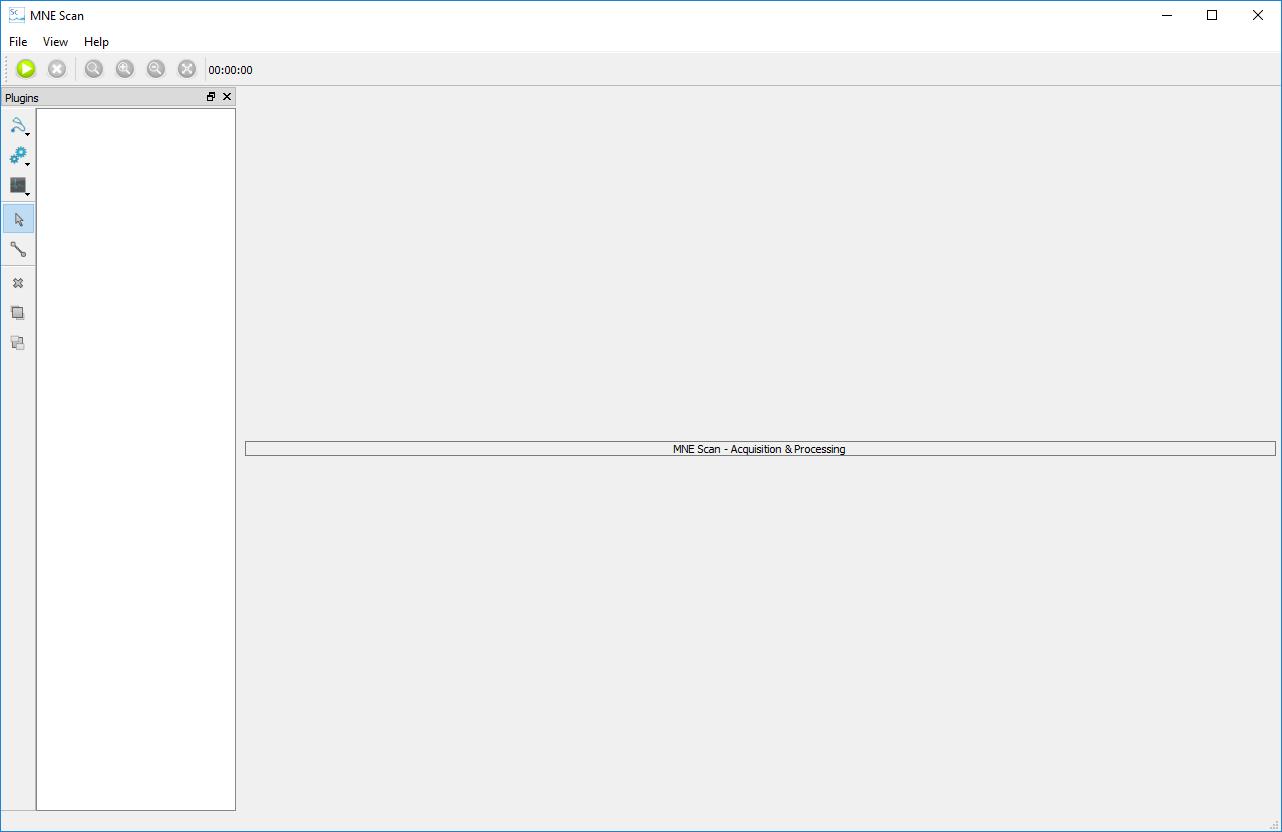
\includegraphics[scale=0.3]{Figures/MNE-Scan.PNG}
	
	\end{center}
	
	\caption{MNE Scan}

\end{wrapfigure}

